\chapter{Architecture Description}

% This doesnt have to be a section
\section{Overall description}

The MANGO project aims at allowing developers to easily develop applications that target different types of accelerator architectures. In particular,  three types of accelerators are considered: symmetric multiprocessors, which are characterized by good capabilities in terms of OS support and execution flexibility (i.e., they are able to run a POSIX-compliant runtime); GPGPU-like accelerators, which are programmable but are not able to run a fully compliant POSIX runtime; and hardware accelerators, which do not need or support any kind  of software runtime. Applications, on the other hand, may be developed either by domain experts with limited knowledge of parallel computing and programming models, or by more experienced programmers. 

Thus, the following requirements arise:
\begin{itemize}
    \item 
    Supporting the use of industry-standard programming models for heterogeneous systems, such as OpenCL, while guaranteeing functional portability across different programmable accelerators, as well as host-side compatibility for all accelerators and automated resource management;
    \item 
    Supporting a simple fork-join model, on which application developers not willing to use OpenCL can map their applications;
    \item
    Supporting future extensions of the MANGO software stack to support skeleton-based programming.
\end{itemize}

The user-facing module (Libmango), therefore, needs to operate in a way that is akin to an intermediate language in a compiler: it must allow the software stack developers to easily map high-level programming models on the range of supported accelerators, while providing at least functional compatibility. Depending on the individual capabilities of each accelerator, the low-level runtime system should also introduce optimizations or additional features; this would indeed cause compatibility issues, but it would also allow developers to implement specialized versions of their applications for any given accelerator. \cite{mango_exploring_manycore_architectures}

%TODO better diagram
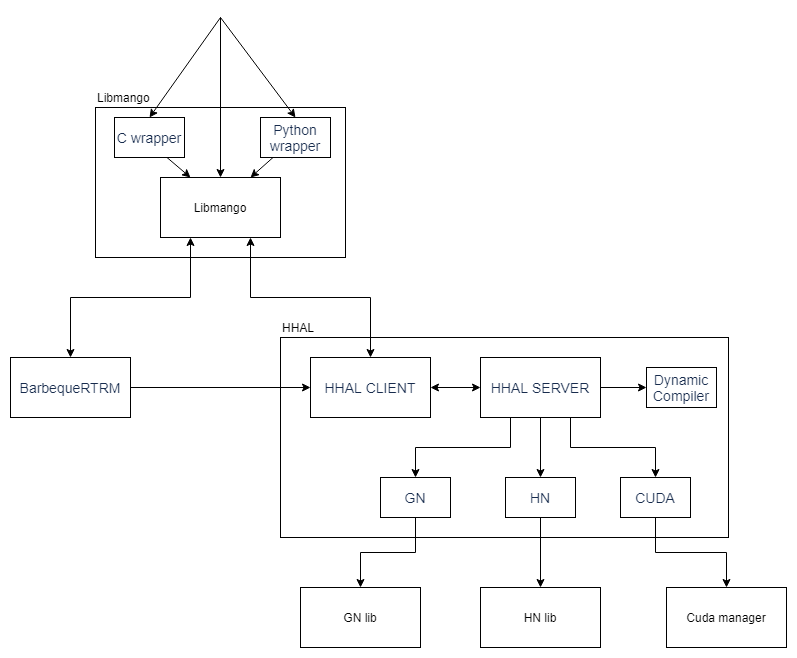
\includegraphics[scale=0.5]{img/architecture.png}

\section{Core elements}
Throughout the multiple MANGO modules, there are a few core elements often present in each module. These are the components necessary to specify and control an user application and its execution. Although their names may vary from module to module, here they are defined as Kernel, Memory Buffer, Event and Task graph.

\subsubsection{Kernel}
In computing, a compute kernel is a routine compiled for high throughput accelerators (such as graphics processing units (GPUs), digital signal processors (DSPs) or field-programmable gate arrays (FPGAs)), separate from but used by a main program (typically running on a central processing unit). \cite{kernel_wikipedia}

The MANGO system manages user defined Kernels and their execution. For a particular Kernel, multiple sources (accelerator specific implementations of the kernel) can be specified. The architectures for which an implementation is available are considered in the kernel-accelerator assignation process by the resource manager. 

As any computer program, a kernel must have the capability of interacting with the outside world in order to perform significant work. This is achieved through the support of kernel arguments.

%TODO styling
Three types of kernel arguments are supported: 
\begin{itemize}
    \item Scalar Argument: A scalar value. For example, an integer.
    \item Buffer Argument: A pointer to a Memory Buffer.
    \item Event Argument: A pointer to an Event data type.
\end{itemize}

\subsubsection{Memory Buffer}
%TODO better diagram
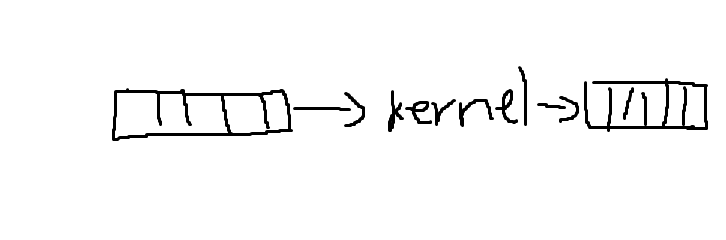
\includegraphics[scale=0.5]{img/kernel_buffer.png}

In computer science, a data buffer (or just buffer) is a region of a physical memory storage used to temporarily store data while it is being moved from one place to another. \cite{buffer_wikipedia}

Kernels read from Input Buffers and write to Output Buffers for inter-kernel and host-kernel data transfering.

A Memory Buffer is defined by the user and allocated by MANGO at the target architectures, where a Kernel that makes use of said Buffer (as either input or output) is assigned.

\subsubsection{Event}

An event is a data structure utilized for communication and synchronization of different parts of the system.

User defined events can be accessed by Kernels through Event Arguments, providing the user with the necessary tools for the implementation of host-kernel or inter-kernel synchronization.

By default, MANGO utilizes kernel termination events for both internal and host synchronization.

\subsubsection{Task Graph}

The Task Graph gives a global picture of the application's behaviour and represents data and control dependencies between Kernels, Memory Buffers and Events. The Task Graph provides the resource manager with the information needed to generate the best feasible resource allocation for the requested QoS. \cite{mango_exploring_manycore_architectures}


\section{Libmango}
Libmango is the front-facing module of the MANGO system, hence providing the system's API for user interaction with the underlying components, and acting as an abstraction layer between user defined models and module specific requirements.

The goal of the Libmango module is to allow software stack developers to easily map high-level programming models on the range of supported accelerators. Through the communication with the BarbecueRTRM and HHAL modules, user models are automatically mapped to the supported accelerators in a transparent manner, removing integration complexity from the user's hands.

The Libmango API allows developers to indicate to the runtime the components of their application, namely kernels, memory buffers and events. These are grouped in a task graph that represents the dependencies among the multiple components. 

Libmango is implemented in the C++ programming language, so its native usage is through the C++ API. However, a set of wrappers for other languages are provided, namely the C and Python API wrappers.

\subsection{Context}
The Context is the main class in the Libmango module, it holds the state information of the host side runtime for a single application, and its created by the user at the beginning of their interaction, with an application name and a recipe file needed by BarbecueRTRM for the resource allocation. Every subsequent component (kernels, buffers, events and task graph) has to be registered in the Context in order to be considered part of the application.

Once the application is specified, the task graph information is sent to the BarbecueRTRM for the resource allocation. After a successful resource allocation, the application is now ready to run.

\subsection{Kernel management}
Libmango exposes functionalities and data structures that can be used to represent and manipulate kernels.

Kernels are identified by an user-provided integer. For a single kernel, multiple implementations can be specified, each one targeting a different supported accelerator and thus provided in their respective architecture's requirements - a kernel implementation targeting an NVIDIA GPGPU would require a CUDA implementation.
Kernel versions (implementations) are stored either in memory or in external files. According to the targeted architecture, multiple source types are supported. The kernel source can be a pre-compiled binary file or code in accelerator-supported language, provided via a string stored in memory or a source file, to be dynamically compiled if required.
The resource manager will rely on the available options in the assignation of kernels to accelerators.

Kernels can be manually started by the developer once the resource allocation is successfully completed.

Libmango supports three types of Kernel arguments: Scalar arguments, Buffer arguments and Event arguments.
These essentially act as wrappers of the HHAL kernel arguments.

\subsubsection{Scalar argument}
A Scalar argument consists of a scalar value. The types supported by Libmango are signed and unsigned integers of sizes 8, 16, 32 and 64; as well as float values.
When a Scalar argument is created, the provided value is copied and stored in memory, and later sent to the HHAL module when their respective kernel is ran. 

\subsubsection{Buffer argument}
A Buffer argument consists of a Buffer integer identifier. The corresponding memory pointer in the accelerator's memory space is passed as an argument to the Kernel at execution time.

%TODO better explain how the kernel function receives the event argument depending on the architecture
\subsubsection{Event argument}
An Event argument consists of an Event integer identifier. The corresponding Event is passed as an argument to the Kernel at execution time.


\subsection{Buffer management}
Libmango exposes functionalities and data structures that can be used to represent and manipulate Memory Buffers. Buffers are the main data communication instruments between the host and the executing Kernels. 

A Buffer is identified by an user-provided integer. It consists of a pointer to a memory location where the Memory Buffer starts, and its size in bytes. 
For creating a Buffer, the user needs to register it to the application's Context. A Buffer is automatically allocated in the same accelerator where the Kernel that writes to, or reads from it, is assigned to by the resource manager.
Once successfully allocated, Libmango permits the writing of the Buffer with host-side data, as well as reading from the Buffer into host memory.


\subsection{Event management}
To provide developers with synchronization capabilities, Libmango exposes Event functionalities.

An Event is identified by an integer generated by Libmango. Events are synchronization data structures with an internal value utilized to indicate the different stages in the process, or in the case of user-defined Events, any denotation the user gives it.

Libmango lets the user define their own Events. These can be passed as arguments to the Kernels (if the target architecture supports them), which allows for user-defined inter-Kernel or host-Kernel synchronization.

By default, Libmango utilizes Events for Kernel termination synchronization. For every registered Kernel, Libmango automatically generates a Kernel-termination Event, which can also be accessed by the developers for waiting until a started Kernel finishes.

\subsection{API Wrappers}
As the core implementation of Libmango is in the C++ programming language, a set of wrappers are provided to complement the C++ API and allow developers to make use of the MANGO system using their programming language of choice.

Besides the native C++ API, Libmango currently exposes C and Python API wrappers.

\subsubsection{C API Wrapper}
The C language API is a wrapper around the C++ API that is provided both for compatibility with C code and for compatibility with the early version of MANGO, which was developed in C.

All the data types in the function prototypes have been made opaque using specific typedef types. This hides to the application some specific types of the machine, such as the size of the memory addresses. In the current MANGO implementation, the used types are mostly uint32\_t, due to the addressing size that is of 32-bit.

The API is divided in 8 groups: initialization and shutdown, kernel loading, task graph definition, task graph registration, resource allocation, kernel launching, synchronization primitives, and data transfer. \cite{mango_exploring_manycore_architectures}

%TODO
\subsubsection{Python API Wrapper}
TODO

\subsection{Sample Application}

In this section we will go over a sample to showcase and explain the Libmango C++ API usage. The sample application consists on the computation of a SAXPY operation (z = ax + y) over two trivially pre-initialized arrays: x and y. 

\begin{lstlisting}[style=CStyle, caption=saxpy.cu]
extern "C" __global__ 
void saxpy(float a, float *x, float *y, float *out, int n) {
  size_t tid = blockIdx.x * blockDim.x + threadIdx.x;
  if (tid < n) {
    out[tid] = a * x[tid] + y[tid];
  }
}
\end{lstlisting}

The target architecture of the sample is CUDA, hence a precompiled binary of the shown CUDA kernel that performs the SAXPY operation is used.

\begin{lstlisting}[style=CStyle, caption=Sample - Includes]
#include <cstddef>
#include <iostream>
#include <memory>

#include <host/context.h>
#include <host/logger.h>
\end{lstlisting}

First we set up the sample with the necessary includes. Regarding Libmango, \textbf{context.h} is the required header that exposes the C++ API. \textbf{logger.h} is also included to access the Libmango logger.

\begin{lstlisting}[style=CStyle, caption=Sample - Definitions]
#define KERNEL 1
#define B1 1
#define B2 2
#define B3 3

// saxpy function matching the CUDA kernel, used to check the results
void saxpy(float a, float *x, float *y, float *o, float n) {
    for (size_t i = 0; i < n; ++i) {
        o[i] = a * x[i] + y[i];
    }
}
\end{lstlisting}

We now define the kernel and buffers integer identifiers, as well as a \textbf{saxpy} function that matches the \textbf{saxpy.cu} kernel computation, we will use it to check the obtained results.

\begin{lstlisting}[style=CStyle, caption=Sample - Initialization]
int main(int argc, char const *argv[])
{
    // Initialization
    mango::mango_init_logger();
    auto mango_rt = mango::Context("cuda_simple", "test_manga_cuda");

    int n = 4096;
    size_t buffer_size = n * sizeof(float);
    float a = 2.5f;
    float *x = new float[n], *y = new float[n], *o = new float[n];

    for (size_t i = 0; i < n; ++i) {
        x[i] = static_cast<float>(i);
        y[i] = static_cast<float>(i * 2);
    }
\end{lstlisting}

%TODO we mention the recipe file here, it will probably get explained under BarbecueRTRM later, so link to that and clarify
At the beginning of the \textbf{main} function, we initialize the logger, and the application's \textbf{Context} is created. For the initialization of the Context, an application name is required: "cuda\_simple", as well as a recipe file name for the BarbecueRTRM resource allocation: "test\_manga\_cuda".

Then, the three buffers we need for the operation are declared. \textbf{x} and \textbf{y} are the input buffers, so they are initialized with known values. \textbf{o} is the output buffer where we will store the results, so there is no need to initialize its data.

\begin{lstlisting}[style=CStyle, caption=Sample - Kernel loading]
    char kernel_path[] = "/opt/mango/usr/local/share/cuda_simple/saxpy";
    auto kf = std::make_shared<mango::KernelFunction>();
    kf->load(kernel_path, mango::UnitType::NVIDIA, mango::FileType::BINARY);
\end{lstlisting}

To load the saxpy kernel binary file, we create a \textbf{KernelFunction} object, and then load the kernel through the \textbf{load()} function, specifying the target architecture and file type.

\begin{lstlisting}[style=CStyle, caption=Sample - TaskGraph registration and resource allocation]
    // Registration of task graph
    auto k  = mango_rt.register_kernel(KERNEL, kf, {B1, B2}, {B3});

    auto b1 = mango_rt.register_buffer(B1, buffer_size, {}, {KERNEL});
    auto b2 = mango_rt.register_buffer(B2, buffer_size, {}, {KERNEL});
    auto b3 = mango_rt.register_buffer(B3, buffer_size, {KERNEL}, {});

    auto tg = mango::TaskGraph({k}, {b1, b2, b3});

    // Resource Allocation
    mango_rt.resource_allocation(tg);
\end{lstlisting}

In order to realize the resource allocation, we first need to register the elements in the Context and create the \textbf{TaskGraph}.
The kernel is registered in the Libmango Context by providing its id, kernel function and input and ouput buffers.
The buffers are registered by providing their ids, size, kernels where they act as input and kernels where they act as output.

Finally, the \textbf{TaskGraph} is created with the previously registered elements and the resource allocation is performed over the specified TaskGraph.

\begin{lstlisting}[style=CStyle, caption=Sample - Arguments set up]
    auto argX = mango::BufferArg(b1);
    auto argY = mango::BufferArg(b2);
    auto argO = mango::BufferArg(b3);
    auto argA = mango::ScalarArg<float>(a);
    auto argN = mango::ScalarArg<int>(n);

    auto argsKERNEL = mango::KernelArguments({argA, argX, argY, argO, argN}, k);
\end{lstlisting}

The \textbf{saxpy} kernel receives five arguments, two scalars and three buffers. A \textbf{BufferArg} is created for each buffer argument, and two \textbf{ScalarArg} are created with their respective types (float and int) for each of the scalar arguments.

A \textbf{KernelArguments} object groups the arguments to be passed to a given kernel in the stated order.

\begin{lstlisting}[style=CStyle, caption=Sample - Writing buffers]
    std::cout << "Sample host: Writing to buffer 1..." << std::endl;
    b1->write(x, buffer_size);

    std::cout << "Sample host: Writing to buffer 2..." << std::endl;
    b2->write(y, buffer_size);
\end{lstlisting}

Before launching the kernel, we need to write the data from the host buffers onto the registered buffers that where allocated at the target accelerators in the resource allocation. To write to a buffer, we use the \textbf{write()} function of the \textbf{Buffer} objects that were returned from the Context registration.
    
\begin{lstlisting}[style=CStyle, caption=Sample - Kernel launch]
    std::cout << "Sample host: Starting kernel..." << std::endl;
    auto e = mango_rt.start_kernel(k, argsKERNEL);

    std::cout << "Sample host: Waiting for kernel completion..." << std::endl;
    e->wait();
\end{lstlisting}

We are now ready to execute the kernel. The \textbf{start\_kernel()} function takes the kernel and its arguments and returns a kernel termination \textbf{Event}. By calling the event's \textbf{wait()} function, the host execution is blocked until the kernel's termination is notified.

\begin{lstlisting}[style=CStyle, caption=Sample - Checking results]
    b3->read(o, buffer_size);

    float *expected = new float[n];
    saxpy(a, x, y, expected, n);

    bool correct = true;
    for (int i = 0; i < n; ++i) {
        if (o[i] != expected[i]) {
            std::cout << "Sample host: Error!\n" << std::endl;
            correct = false;
            break;
        }
    }
    if(correct) {
        std::cout << "Sample host: SAXPY correctly performed!" << std::endl;
    }
\end{lstlisting}

Once the kernel terminated, we can read the results from the output buffer \textbf{b3}. By using the buffer's \textbf{read()} function, we can read the data from the accelerator's memory into the \textbf{o} host buffer.

We use the \textbf{saxpy} function defined at the beginning of the sample to check the correctness of the results.

\begin{lstlisting}[style=CStyle, caption=Sample - Teardown]
    mango_rt.resource_deallocation(tg);
    delete[] x;
    delete[] y;
    delete[] o;
    delete[] expected;

    return 0;
}
\end{lstlisting}

Before returning, we perform the resource deallocation of the TaskGraph, and free the host buffers.

\section{BarbecueRTRM}

\section{HHAL}

\section{CUDA Manager}

\section{HN}

\section{GN}